\chapter{Arsenal Numérico}

Empecemos equipándonos de algunas armas elementales muy 
frecuentes en los problemas de olimpiada.

Este capítulo en particular tiene una gran intersección 
con todas las áreas de la olimpiada, pero creo que se puede 
encasillar más en teoría de números.

\section{Criterios de Divisibilidad}

Los criterios de divisibilidad son reglas que sirven para saber 
si un número es divisible por otro (ahorrándonos una 
que otra división).

\begin{enumerate}[i.]
    \item \textbf{Criterio del 2.} Un entero \( a \) es divisible 
    por 2 si y sólo si \( a \) termina en cifra par.
    \item \textbf{Criterio del 3.} Un entero \( a \) es divisible 
    por 3 si y sólo si la suma de las cifras de \( a \) es 
    divisible por 3.
    \item \textbf{Criterio del 4.} Un entero \( a \) es divisible 
    por 4 si y sólo si el número formado por las dos últimas cifras 
    es divisible por 4.
    \item \textbf{Criterio del 5.} Un entero \( a \) es divisible 
    por 5 si y sólo si \( a \) termina en 0 o 5.
    \item \textbf{Criterio del 6.} Un entero \( a \) es divisible 
    por 6 si y sólo si \( a \) es divisible por 2 y 3. Es decir, 
    que \( a \) termine en 0, 2, 4, 6 o 8, y al mismo tiempo que 
    la suma de sus dígitos sea divisible por 3.
    \item \textbf{Criterio del 7.} NO \minitisca.
    \item \textbf{Criterio del 8.} Un entero \( a \) es divisible 
    por 8 si y sólo si el número formado por las tres últimas 
    cifras es divisible por 8.
    \item \textbf{Criterio del 9.} Un entero \( a \) es divisible 
    por 9 si y sólo si la suma de las cifras de \( a \) es 
    divisible por 9.
    \item \textbf{Criterio del 10.} Un entero \( a \) es 
    divisible por 10 si y sólo si \( a \) termina en 0.
    \item \textbf{Criterio del 11.} Un entero \( a \) es 
    divisible por 11 si y sólo si la diferencia de la suma de 
    las cifras en posición impar de \( a \) menos la suma de las 
    cifras en posición par de \( a \) es divisible por 11.
\end{enumerate}

\begin{exercise}
    ¿Es cierto que si un número natural es divisible por $4$ y 
    $3$, entonces es divisible por $12$?¿Por qué?
\end{exercise}

\begin{exercise}
    ¿Es cierto que si un número natural es divisible por $4$ y 
    $3$, entonces es divisible por $12$?¿Por qué?
\end{exercise}

\begin{question}
    ¿Notas algo?
\end{question}

\section{Fuérzalo}

Seguido te encontrarás con problemas donde va a ser necesario 
encontrar un número tal que al multiplicarlo o sumarlo con otro 
te dé alguna condición especial. Aquí es muy útil que hagas las 
operaciones en vertical como te lo han enseñado en la escuela y 
que veas qué números necesitas para obtener un resultado 
específico.

\begin{exercise}
    Un número se dice \textit{capicúa} si se lee igual al 
    derecho que al revés. Por ejemplo: 1221, 838. Encuentra el 
    menor entero que le tienes que sumar a 25973 para que el 
    resultado sea un número \textit{capicúa}.
\end{exercise}

\begin{exercise}
    Encuentra el menor número que al multiplicar por 7, el 
    resultado sea un número que termina en 216. (Es decir, que 
    sus últimos tres dígitos sean 2, 1, 6, en ese orden).
\end{exercise}

\section{Suma de Gauss}

La sumatoria de Gauss es muy útil por lo que significa y por la 
versatilidad de su demostración. La suma de Gauss nos permite 
encontrar la suma de los primeros \(n\) números. Antes de que 
empieces, te invito a que encuentres una manera fácil de obtener 
la suma de todos los números del 1 al 100 sin tener que calcular 
todas las sumas.

\[
1+2+3+\dots+n = ?
\]

\begin{exercise}
    En una fiesta, el anfitrión recibe a 100 invitados que van 
    llegando de uno por uno. Si cada invitado saluda al anfitrión 
    y a todos los otros invitados que llegaron antes que él, 
    ¿cuántos saludos hubo? (Ninguna pareja de personas se saludó 
    más de una vez).
\end{exercise}

\begin{exercise}
    Calcula la suma \(3 + 6 + 9 + \dots + 300\).
\end{exercise}

\begin{exercise}
    Alfredo leyó un libro. El primer día leyó 5 páginas, y cada 
    día siguiente leyó 2 páginas más que el anterior. Si la 
    lectura le llevó un total de 20 días, 
    ¿cuántas páginas tenía el libro?
\end{exercise}

\section{Ciclos}

Algunas veces te pedirán encontrar algún término de una serie. Para lo cual es muy importante que identifiques qué relación numérica está expresada en la serie.

En otras ocasiones se les pide a los alumnos encontrar el último dígito de alguna expresión o de una operación muy grande. Generalmente esas expresiones tienen algún ciclo y es muy sencillo encontrar lo que se pide.

Finalmente, hay ocasiones en que se te pide encontrar algún término en una serie, que se cicla dada ciertos términos. Para esto es bueno que siempre intentes encontrar algunos términos iniciales.

\begin{exercise}
    Encuentra el último dígito de \( 44^{4444} \).
\end{exercise}

\begin{exercise}
    Encuentra los últimos dos dígitos de \( 3^{1234} \).
\end{exercise}

\begin{exercise}
    Fátima escribe los números pares en una fila: 2468101214… 
    ¿Qué dígito está en la posición 2016? ¿A qué número 
    corresponde? Por ejemplo, en la posición 8 hay un dígito 2 
    que corresponde al número 12.
\end{exercise}


\section{Bonus}

El criterio de divisibilidad del 7 es \textit{horrible} y dice 
que un número es divisible entre 7 si el número que resulta de 
borrar el último dígito y restarlo dos veces también es 
divisible entre 7 (es más rápido y sencillo hacer la división).

\subsection{Notación Científica}

Se llama así a cuando expresamos un número de la forma:

\[
a_0\cdot 10^0 + a_1\cdot 10^1+a_2\cdot 10^2+\dots a_n\cdot 10^n
\]

Así es como funciona el sistema decimal, el que usamos.

Expresar los números de esta forma es muyyyy útil (te percatarás 
al resolver los problemas) y es una estrategia que debe estar 
en nuestra mente acompañándonos siempre.

\newpage

\section{Problemas}

Cada problema que resuelvas te dará el número de treboles 
que especifica ($x \clubsuit$), ¡colecta los más que puedas!

\epigraph{La matemática es la reina de las ciencias y la teoría de 
números es la reina de las matemáticas}{Carl Friedrich Gauss, el 
Príncipe de los Matemáticos}

\begin{problem}[$2 \clubsuit$]
    Para que el número de $7$ cifras $6a74b14$ sea múltiplo de 
    $9$ y de $11$, ¿cómo deben ser $a$ y $b$? 
\end{problem}

\begin{problem}[$2 \clubsuit$]
    De los números del 1 al 9, el único que no divide a 2016 
    es el 5. Si reordenas los dígitos del 2016 puedes
    obtener un número que, de los números del 1 al 9, únicamente 
    no es divisible entre 7. ¿Cuál es ese número?
\end{problem}

\begin{problem}[$3 \clubsuit$]
    Encuentra un número que termine en 6 y tal que si le 
    quitas ese último dígito (el 6) y lo colocas en el 
    principio (por ejemplo, el 126 pasaría a ser 612), el 
    nuevo número es 4 veces el número original.
\end{problem}

\begin{problem}[$3 \clubsuit$]
    El número de cinco dígitos distintos \(2abcd\) cumple que 
    \(2abcd \times 4 = dcba2\). (Los dígitos son \(2,a,b,c,d\)). 
    Además, sabemos que \(2abcd\) es múltiplo de 72. 
    Encuentra el número.
\end{problem}

\begin{problem}[$3 \clubsuit$]
    ¿Existe algún número de 6 dígitos divisible por 11 que 
    tenga como dígitos 1, 2, 3, 4, 5 y 6 en algún orden 
    (especifica cual en caso de que si)?
\end{problem}

\begin{problem}[$3 \clubsuit$]
    Louis tiene cierta cantidad de dinero y está conformada por 
    los dígitos 2, 4, 1, 5, 3 y 3, en algún orden. La cantidad es 
    múltiplo de 8, 9 y 11. ¿Cuál es la menor cantidad de dinero 
    que puede tenerr Louis?
\end{problem}

\begin{problem}[$3 \clubsuit$]
    Se forman tres números enteros de tres cifras 
    \(abc,def,ghi\), donde cada letra representa un dígito del 
    1 al 9 sin que se repitan. Si la suma de los tres números 
    termina en 65, ¿cuál es el valor de dicha suma?
\end{problem}

\begin{problem}[$3 \clubsuit$]
    Encuentra el menor número a que cumple que $a + 2a + 3a + 
    4a + 5a + 6a + 7a + 8a + 9a$ es un número con todas sus 
    cifras iguales.
\end{problem}

\begin{problem}[$3 \clubsuit$]
    (1), (2,3), (4,5,6), (7,8,9,10), (11,12,13,14,15) … 
    ¿Cuántos números tiene el paréntesis que contiene al número 
    2017?
\end{problem}

\begin{problem}[$3 \clubsuit$]
    El abuelo repartirá 2007 monedas entre sus nueve nietos 
    (podemos llamarlos A, B, C, D, E, F, G, H, I) de la 
    siguiente manera: los sienta alrededor de una mesa en el 
    orden de sus nombres y va entregando en el mismo orden una 
    moneda a cada uno, empieza con A; al completar la vuelta, la 
    siguiente vuelta comienza con el último; es decir, le 
    entrega una más a I y continúa con A, entregando moneda por 
    moneda; termina la siguiente vuelta con H, le entrega su 
    moneda y con él mismo inicia la siguiente vuelta. Procede de 
    esta manera hasta haber repartido todas las monedas. 
    ¿Cuántas monedas le quedan a cada nieto? ¿A qué nieto le 
    entregó la última moneda?
\end{problem}

\begin{problem}[OMMEB 2017, $4 \clubsuit$]
    El número \(100...00200...001\) se formó con un \(1\) 
    seguido de \(2017\) ceros, luego un \(2\), seguido de otros 
    \(2017\) ceros y al final un \(1\). ¿Cuántos ceros tiene 
    la raíz cuadrada del número?
\end{problem}

\begin{problem}[OMMEB 2017, $5 \clubsuit$]
    ¿Cuántos enteros de dos dígitos existen tales que al 
    multiplicarlos por \(3\) se obtiene un número de tres 
    dígitos todos ellos iguales?
\end{problem}

\begin{dproblem}[$3 \clubsuit$]
    Encuentra una fórmula para la suma de los primeros 
    $n$ números impares
\end{dproblem}

\begin{dproblem}[$3 \clubsuit$]
    Encuentra una fórmula para la suma de los primeros 
    $n$ números pares
\end{dproblem}

\begin{problem}[$3 \clubsuit$]
    Encuentra la suma de todos los números de cinco cifras en 
    los que los dígitos 1, 2, 3, 4, 5 aparecen exactamente una 
    vez.
\end{problem}

\begin{remark}
    Una vez resuelto ese problema, es más sencillo atacar 
    el problema $Y$ del capítulo "Conteo I".
\end{remark}

\begin{problem}[OMMEB 2017, $4 \clubsuit$]
    Una pulga salta sobre los vértices de un polígono regular 
    de \(2017\) lados numerados consecutivamente desde \(1\) 
    hasta \(2017\). La pulga inicia en el vértice \(6,\) siempre 
    salta cuatro vértices hacia adelante pero se regresa dos 
    vértices cuando cae en uno numerado como potencia de dos 
    (por ejemplo después del salto a \(20,\) regresa al \(18.\)). 
    ¿Después de cuántos saltos supera por primera vez el número 
    \(1?\)
\end{problem}

\begin{problem}[OMMEB 2017, $4 \clubsuit$]
    Se colocan los números impares \(3,\) \(5,\) \(7,\) 
    \(9,\ldots,\) siguiendo una espiral como se muestra en la 
    figura. El número \(3\) quedó en un primer cuadrado de 
    \(1 \times 1,\) al poner el \(9,\) se cerró un segundo 
    cuadrado de \(2\times 2,\) un tercer cuadrado se cerró al 
    poner el \(19.\) ¿Qué número cierra el cuadrado número \(18?\)
\end{problem}

\begin{figure}[h]
    \centering
    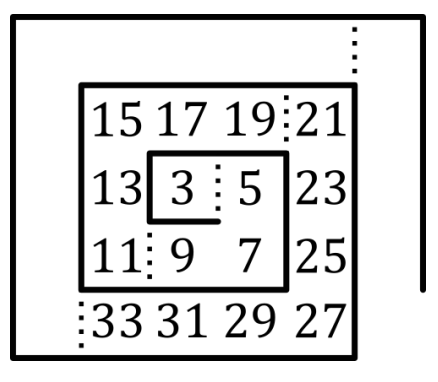
\includegraphics[height=3cm]{17OMMEBN1EP3.png}
\end{figure}

\begin{problem}[$3 \clubsuit$]
    Demuestra el criterio de divisibilidad del $2$.
\end{problem}

\begin{problem}[$4 \clubsuit$]
    Demuestra el criterio de divisibilidad del $3$.
\end{problem}

\begin{problem}[$3 \clubsuit$]
    Demuestra el criterio de divisibilidad del $4$.
\end{problem}

\begin{problem}[$3 \clubsuit$]
    Demuestra el criterio de divisibilidad del $5$.
\end{problem}

\begin{problem}[$4 \clubsuit$]
    Demuestra el criterio de divisibilidad del $9$.
\end{problem}

\begin{problem}[$4 \clubsuit$]
    Demuestra el criterio de divisibilidad del $11$.
\end{problem}

\begin{dproblem}[$4\clubsuit$]
    Encuentra el criterio de divisibilidad de $2^x$ y demuestra 
    porqué funciona.
\end{dproblem}

\begin{problem}[$6 \clubsuit$]
    Demuestra el criterio de divisibilidad del $7$.
\end{problem}

\begin{problem}[$7 \clubsuit$]
    \jp 
    Encuentra un criterio de divisibilidad generalizado para 
    todo número primo y demuestra porqué funciona .
\end{problem}

\noindent El máximo número de $\clubsuit$ en este capítulo es de 
$92 \clubsuit$.
